\chapter{Architettura del framework}
\label{capitolo3}
\thispagestyle{empty}
In questo capitolo verr\`a descritta l'architettura del framework sviluppato durante il lavoro di tesi. Inizialmente presenteremo la piattaforma Neosperience \textit{Engage} specificando dove si colloca il nostro lavoro al suo interno. In seguito mostreremo quali sono i moduli progettati e le soluzioni proposte per ogni fase della data analysis. Affronteremo quindi le sfide di raccolta, preparazione e conversione dei dati, fino all'esecuzione degli algoritmi di clustering. Infine, verr\`a presentato un \textit{workflow} modulare dell'intera architettura, utile per una visione d'insieme degli strumenti disponibili.
\section{Neosperience Engage}
Neosperience \`e una azienda italiana che offre servizi di marketing e \textit{customer experience}. In un mercato globale \mbox{iper-competitivo} e \mbox{iper-connesso}, per contrastare la crescente dispersione degli utenti, un marchio deve stabilire un legame individuale con il cliente. Customer experience descrive la percezione che il cliente matura---razionalmente ed emotivamente---della relazione con il marchio. Di conseguenza, la gestione dell'\textit{esperienza cliente} \`e la pianificazione e la risposta alle interazioni con il consumatore, al fine di raggiungerne ed eccederne le aspettative ed in questo modo aumentare la soddisfazione, la lealt\`a e il sostegno del cliente al marchio\footnote{``The practice of designing and reacting to customer interactions to meet or exceed customer expectations and, thus, increase customer satisfaction, loyalty and advocacy'' - Gartner}: in una parola, coinvolgimento o \textit{engagement}. L'esperienza cliente \textit{digitale} apre nuove vie di contatto con le persone: non solo portali internet, ma applicazioni per social network e dispositivi mobili, tecnologie 3D e negozi virtuali, realt\`a aumentata e \textit{gamification}. Il ciclo vitale di un cliente rispetto ad un marchio inizia con la scoperta di un prodotto o un servizio; dopo questo primo contatto, seguono diversi \textit{moment of truth}, le occasioni in cui il cliente interagisce con l'azienda e si forma una opinione, consapevole ed inconscia. Il mantenimento del cliente dipende dalla capacit\`a del marchio di influire positivamente in ciascuno di questi istanti: la valutazione del prodotto, la decisione dell'acquisto e l'esperienza d'uso. Questo non \`e solo qualit\`a del servizio, ma arrivare ad una comprensione cos\`i profonda dell'utente da poter offrire una esperienza---contenuti e benefici---tanto personalizzata ed appagante da indurlo non solo a restare leale al marchio ma a convincere altri ad avvicinarsi. Per raggiungere questo grado di conoscenza \`e necessario estrarre indizi da ogni punto di contatto con il cliente, sfruttando l'immensa mole di informazione nella Rete.\\
Recentemente, Neosperience ha sviluppato Engage, uno strumento che permette di creare un negozio virtuale i cui prodotti sono ordinati secondo la significativit\`a che essi hanno per l'utente che li sfoglia. In particolare, una applicazione costruita con Engage \`e una galleria di contenuti, al cui interno ciascun prodotto \`e presentato su una \textit{card}, ovvero un volantino digitale che racchiude una intestazione, una immagine e una breve descrizione testuale. Ad ogni card viene associato il profilo del cliente ideale o \textit{target} che, in base ad indagini di mercato, \`e ritenuto essere il miglior acquirente del prodotto. Il target \`e definito mediante variabili demografiche (et\`a, genere, luogo di nascita, istruzione), interessi e geolocazione (la distanza dal negozio fisico).
La piattaforma Engage, sottostante all'applicazione, recupera i dati personali dell'utente (da Facebook, Twitter e Foursquare) delineando quindi un profilo unico che lo contraddistingue. Partendo da questo profilo, Engage misura, per ogni oggetto nel catalogo, la somiglianza tra il target dell'oggetto e l'utente dell'applicazione, in modo tale che i prodotti vengano riordinati e visualizzati in ordine di significativit\`a.\\
Il nostro lavoro \`e stato motivato dall'esigenza di Neosperience di valorizzare i dati degli utenti raccolti tramite la propria piattaforma Engage. Questi dati difatti racchiudono il potenziale per un diverso approccio alla segmentazione della clientela, facendo leva su informazioni variegate, semi-strutturate e non strutturate, ma nuove e complementari rispetto alle tradizionali categorie sociali e geografiche. L'opportunit\`a offerta da questi dati \`e la conoscenza puntuale degli interessi, delle opinioni, del mood di ciascun cliente, e la possibilit\`a di rispondervi in tempo reale.
%, limitati soltanto dalla capacit\`a di elaborare e assimilare questa informazione.
\subsection{Il modello dei dati}
Nel progetto originale, Engage \`e alimentato da tre sorgenti di dati: Facebook, Twitter e Foursquare.\\
\textbf{Facebook}, con oltre un miliardo di utenti mensili, \`e il pi\`u diffuso e noto social network al mondo. In Facebook, un utente pu\`o pubblicare la propria storia personale, interessi, esperienze, foto, lavoro e perfino stati d'animo. D'altronde, il fulcro dei social network \`e tessere relazioni, e Facebook non fa eccezione: ogni utente pu\`o stringere amicizia con altri utenti, condividere con essi contenuti, conversare, giocare, organizzare eventi ed essere informato di ogni cambiamento nella propria rete sociale. Fra le tre sorgenti, Facebook contribuisce la porzione dominante di informazione: il profilo utente, i like, le amicizie. Come riportato in \autoref{fig:modello_dati}, la frazione osservabile del profilo include il nome, il genere, la data e il luogo di nascita, la citt\`a di residenza, l'istruzione (scuola superiore, universit\`a e formazione specialistica), lo stato sentimentale e l'orientamento sessuale. Al pari di ogni altro nodo del grafo sociale di Facebook, i like sono identificati univocamente e organizzati in oltre 200 macrocategorie, talvolta ulteriormente frazionate in sottogruppi: questo ha permesso di ridurre notevolmente la dimensionalit\`a del problema.

\textbf{Twitter} \`e un social network e una piattaforma di microblogging. Al cuore di Twitter vi sono i \textit{tweet}, brevi messaggi in 140 caratteri che un utente pubblica e la piattaforma notifica a tutti i suoi contatti, chiamati \textit{follower}. Un utente riceve i tweet delle persone che segue sulla propria bacheca o \textit{home timeline}, da cui pu\`o rispondere, inserendosi nel flusso di tweet esistente, o ripubblicare (\textit{retweet}), propagando il tweet ai propri follower. Per organizzare tematicamente le conversazioni, i tweet sono spesso etichettati con un \textit{hashtag}, una parola chiave preceduta da un cancelletto, o \textit{hash} in inglese. Questa convenzione nacque spontaneamente tra gli utenti di Twitter e fu raccolta ed integrata nella piattaforma, che oggi pubblica in tempo reale la lista dei \textit{trending topics}, le parole o argomenti di discussione che compaiono pi\`u frequentemente negli ultimi tweet.

\textbf{Foursquare} \`e tanto un social network focalizzato sulla posizione dell'utente quanto un gioco, il cui successo \`e indubitabilmente connesso al dilagare di dispositivi mobili e intelligenti, sempre pi\`u comunemente provvisti di una antenna GPS. Foursquare non solo rende pubblica la posizione dell'utente, permettendo di trovare gli altri utenti nella medesima zona, ma invita gli iscritti a registrarsi (\textit{check in}) ai luoghi di incontro che visitano---un negozio, un bar, un museo---e attribuisce punti e distintivi (\textit{badges}) per premiare la frequenza con cui vi si accede o la scoperta di nuovi luoghi prima dei propri amici.
\begin{figure}[h]
    \centering
    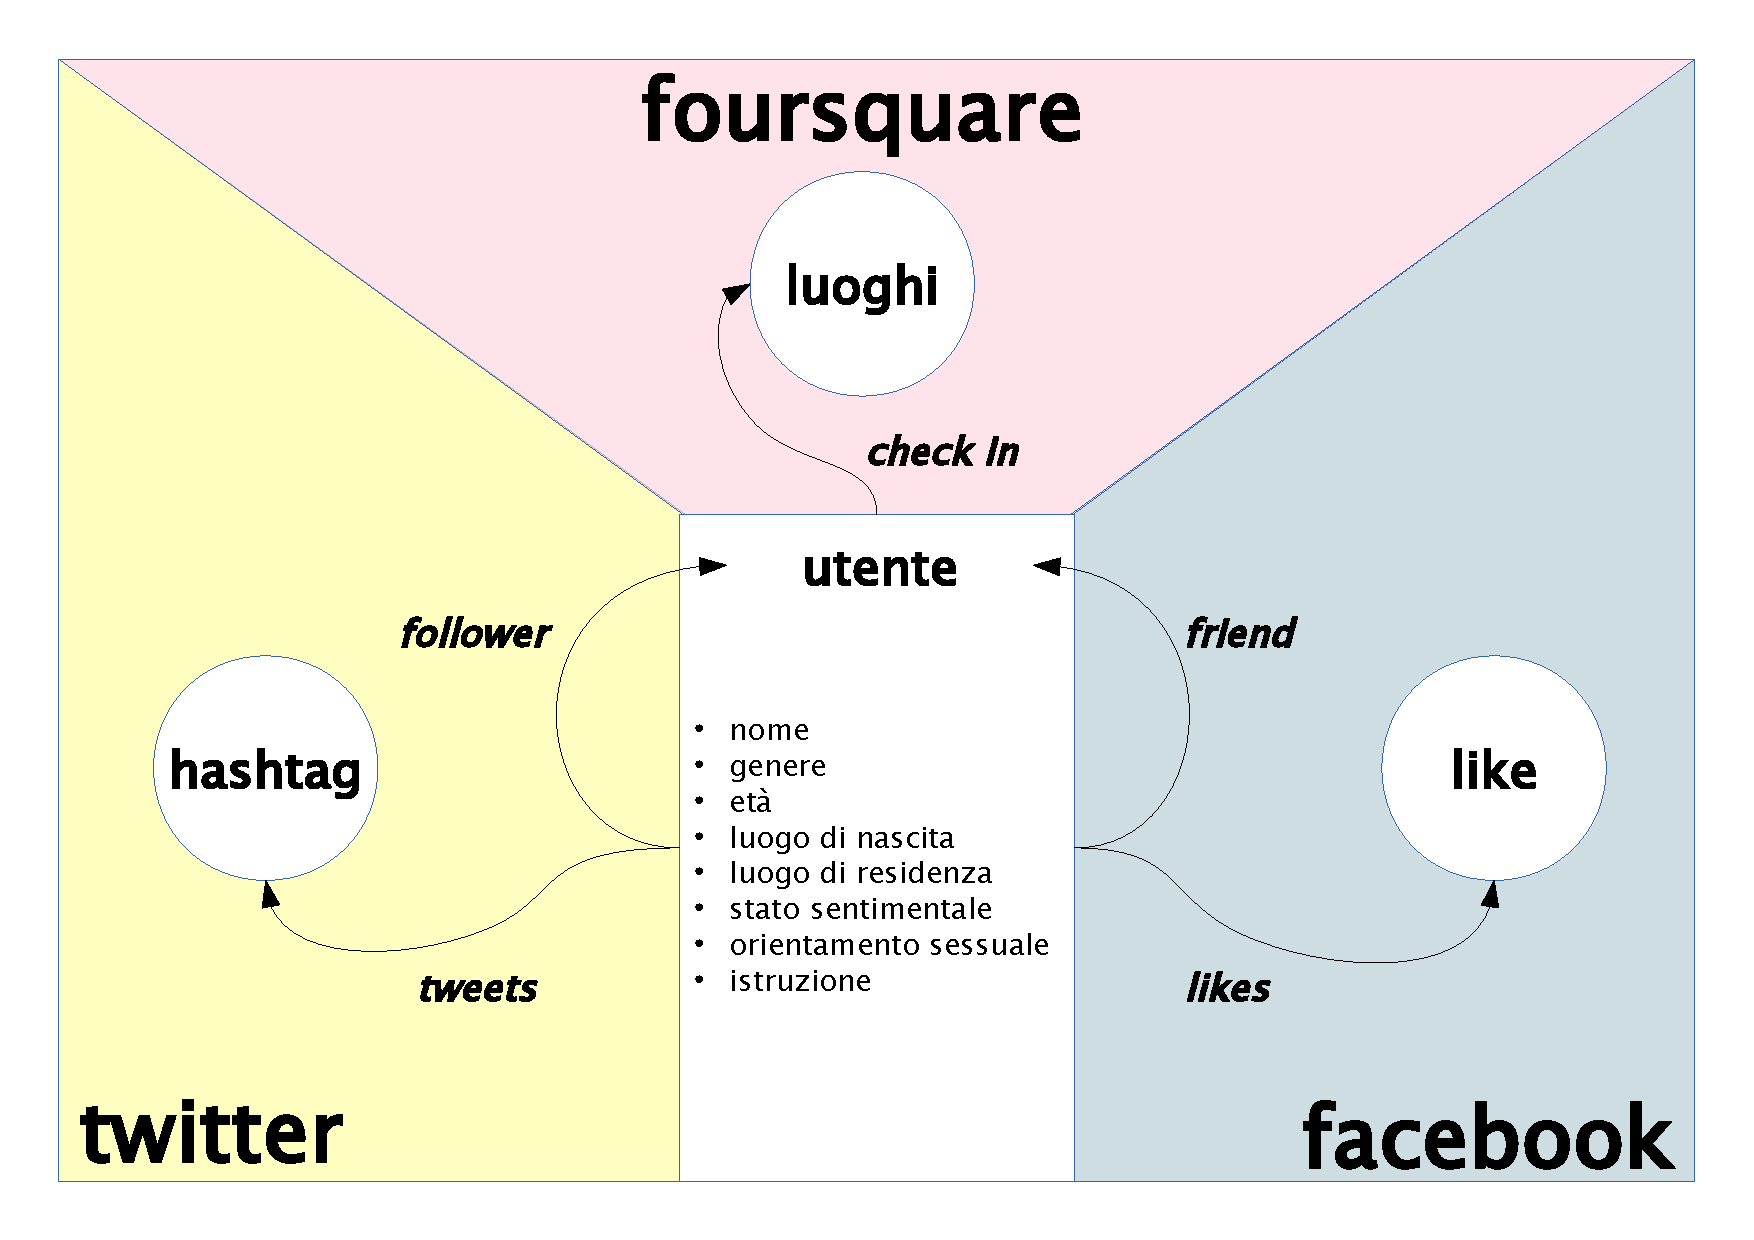
\includegraphics[width=0.95\textwidth]{pictures/modello_dati.pdf}
    \caption{Modello dei dati}
    \label{fig:modello_dati}
\end{figure}
\subsection{Problematiche di integrazione fra le sorgenti}
L'obiettivo finale \`e definire un modello unico dei dati, come esposto in \autoref{fig:modello_dati}, per integrare tre sorgenti eterogenee.\\
Una evidente differenza fra Twitter e Facebook \`e la natura e lo scopo delle interazioni fra gli utenti. Facebook \`e solitamente usato per stare in contatto con persone che si conosce nella vita reale e ritrovare chi si \`e frequentato nel passato. In particolare, una volta stretta amicizia il rapporto tra due amici \`e paritario e simmetrico: possono scambiarsi liberamente messaggi ed ogni contenuto pubblicato da una parte viene notificato all'altra. Al contrario, Twitter \`e principalmente adoperato per comunicare con persone con le quali, pur non frequentandole nella vita reale, si condividono interessi o argomenti di discussione. Questo legame pi\`u superficiale incide sul grado di omofilia nella rete: individui connessi come \textit{friend} saranno in genere pi\`u simili di individui connessi come \textit{follower}, tanto pi\`u se la relazione non \`e reciproca. Twitter realizza un modello asimmetrico di relazione, in cui la discrepanza tra il numero di persone che ci seguono e quelle che seguiamo determina la reputazione dell'individuo all'interno della comunit\`a. Nella pratica, l'asimmetria limita i privilegi del \textit{follower} che, ad esempio, non pu\`o contattare unilateralmente le persone che segue, a meno che non sia stato esplicitamente autorizzato o la relazione sia stata ricambiata. Questa peculiarit\`a ha sensibili implicazioni sul modello dei dati, giacch\'e il grafo degli utenti deve adesso contenere archi orientati.\\
Una ulteriore peculiarit\`a risiede nel confronto tra \textit{like} e \textit{hashtag}. Mentre la relazione tra un utente Facebook e un like \`e binaria---o l'utente ha espresso il proprio gradimento di un oggetto o non lo ha fatto---nel caso di Twitter un utente pu\`o non adoperare mai un hashtag o usarlo con frequenza. Anche in questo caso il modello dei dati richiede una estensione, tramite l'introduzione di pesi sugli archi utente-hashtag. A differenza del caso precedente, dove un arco non orientato pu\`o essere equivalentemente modellato da una coppia di archi orientati, conciliare gli archi privi di peso di Facebook con quelli pesati di Twitter richiede una normalizzazione arbitraria dei pesi. In aggiunta, il significato di un hashtag \`e tutt'altro che analogo ad un like, poich\'e, avendo fissato l'argomento, un tweet pu\`o esprimere tanto apprezzamento quanto avversione, discussione o ``inutile chiacchiera''\footnote{\url{http://web.archive.org/web/20110715062407/www.pearanalytics.com/blog/wp-content/uploads/2010/05/Twitter-Study-August-2009.pdf}}. Per amalgamare semanticamente i tweet ai like sarebbe necessario discriminare i tweet in semplici categorie---\textit{like} e \textit{dislike}---che tuttavia \`e un problema di elaborazione del linguaggio naturale e clustering in s\'e. Infine, la vita media di un hashtag \`e di gran lunga pi\`u breve rispetto ad un like. In termini assoluti, mentre un like \`e sostenuto da un contenuto---una pagina o una realt\`a esterna a Facebook---la creazione di un hashtag richiede al pi\`u uno sforzo di immaginazione; la controparte della proliferazione degli hashtag \`e proprio la loro volatilit\`a. In termini relativi, il carattere episodico e conversevole del tweet richiede tempi di elaborazione ed azione pi\`u stringenti, in quanto l'associazione e il coinvolgimento dell'utente rispetto ad un hashtag pu\`o rapidamente consumarsi. In sintesi, l'analisi dei tweet richiede algoritmi tolleranti di una elevatissima dimensionalit\`a, coerente con l'elaborazione del linguaggio naturale, possibilmente basati su grafi e che garantiscano una bassa complessit\`a temporale anche a scapito della qualit\`a.\\
In ultimo, Foursquare \`e un servizio unico nel suo genere e, contribuendo informazione nuova e non ridondante, non richiede sforzi addizionali di assimilazione nel modello.\\
Una volta definiti i criteri di integrazione, l'ultimo passo sarebbe la \textit{entity resolution} ovvero l'identificazione dei profili che, bench\'e apparentemente scorrelati e provenienti da sorgenti diverse, appartengono al medesimo individuo reale.\\
La quantit\`a di dati a disposizione di Neosperience si \`e rivelata, comunque, molto al di sotto del volume prospettato a regime, sul quale gli algoritmi e le tecniche di data mining avrebbero dovuto essere messe alla prova. Pertanto, il lavoro si \`e articolato nei seguenti passi:
\begin{itemize}
\item \hyperref[raccolta_dati]{raccolta dei dati}
\item \hyperref[selezione_algoritmi]{selezione degli algoritmi}
\item \hyperref[preparazione_dati]{preparazione dei dati}
\item \hyperref[esecuzione_algoritmi]{esecuzione degli algoritmi}
\item \hyperref[capitolo4]{analisi dei risultati}
\end{itemize}
\section{Raccolta dei dati}
\label{raccolta_dati}
Le \mbox{Graph API}\footnote{\url{https://developers.facebook.com/docs/graph-api}} sono lo strumento principale che permette di leggere e scrivere sul grafo sociale di Facebook. Il grafo sociale \`e una rappresentazione delle informazioni presenti nel social network composto da:
\begin{itemize}
\item \textbf{nodi}: entit\`a di vario tipo come utenti, foto, eventi, pagine o commenti, etichettati da un identificatore unico
\item \textbf{archi}: connessioni esistenti tra le entit\`a: relazioni d'amicizia tra utenti, foto in una pagina, commento su certo un evento, etc.
\item \textbf{campi}: attributi delle entit\`a come il compleanno di un utente o il nome di una pagina.
\end{itemize}
La maggior parte delle richieste fatte con le Graph API necessita di un \textit{access token}, che consente un accesso temporaneo e sicuro alle informazioni di profilo di un utente. In particolare, l'access token deve essere composto con una serie di permessi a seconda di quale attributo si vuole leggere o scrivere: ad esempio, se si \`e interessati al nome, al genere e agli amici di un certo individuo, esso deve essere considerare, simultaneamente, i permessi \texttt{user\_about\_me}, \texttt{user\_gender} e \texttt{user\_friends}.\\
Per recuperare queste informazioni \`e sufficiente una chiamata al metodo \texttt{HTTP GET}:
\begin{lstlisting}[basicstyle=\normalfont\ttfamily\scriptsize,backgroundcolor=\color{background}]
GET https://graph.facebook.com/me?fields=name,gender,friends
\end{lstlisting}
che restituisce il seguente file JSon\footnote{JavaScript Object Notation, \url{http://www.json.org}}:
\begin{lstlisting}[language=json,firstnumber=1]
{
  "name": "Nicola P.", 
  "gender": "male",
  "friends": {
    "data": [
      { "name": "Linda",  "id": "987654321" },
      {	"name": "Matteo", "id": "123123123" }
    ]
   }
}
\end{lstlisting}

\subsection{Applicazione per la raccolta dei dati}
Mediante l'SDK per PHP\footnote{\url{https://developers.facebook.com/docs/reference/php/4.0.0}} abbiamo creato un'applicazione che ha ci permesso di recuperare da un utente le seguenti tipologie d'informazione: \textit{profilo} (data di nascita, genere, orientamento sessuale, stato sentimentale, citt\`a natale, citt\`a di residenza  e istruzione), \textit{like} (tutte le pagine su cui si \`e indicato \textit{like}) e \textit{amici} (profilo e like degli amici).\\
L'applicazione \`e stata utilizzata da 87 utenti (che abbiamo indicato con il termine \textit{DAU} o \textit{Direct User Application}) ottenendo, in totale, circa 25 mila profili Facebook in formato JSon.\\
Il passo successivo \`e stato quello di unificare tutti i profili in un unico file GML\footnote{Il formato GML (Graph Modelling Language) permette la rappresentazione dettagliata di un grafo con attributi}. Dal file JSon di ogni DAU sono stati recuperati gli identificatori degli amici e quindi i file JSon ad essi corrispondenti: in questa maniera \`e stato possibile costruire la rete personale del DAU (o \textit{ego-network}) arricchita dalle informazioni di profilo e dai like di ogni nodo. La composizione incrementale di queste reti ha portato alla creazione del grafo finale.

%\subsubsection{Pulizia preliminare dei nodi}
%Il grafo \`e stato ripulito da un insieme di nodi problematici sotto due aspetti. Un utente, infatti, viene escluso se: (1) il numero di attributi di profilo mancanti \`e maggiore della met\`a, e (2) se presenta un valore mancante per un certo attributo e la percentuale dei suoi vicini che, per lo stesso attributo hanno valore mancante, \`e maggiore del cinquanta percento. Il primo punto \`e di immediata comprensione, il secondo \`e giustificato dal fatto che l'inferenza di un certo attributo di un utente \`e basata sui valori che quell'attributo possiede nei vicini dell'utente stesso: se pi\`u della met\`a dei vicini hanno un valore mancante allora \`e lecito pensare che l'inferenza pu\`o addurre risultati molto approssimativi.

\subsection{Creazione dei sottografi}
\label{sampler}
Come gi\`a accennato in precedenza, abbiamo sviluppato un tool\footnote{Il linguaggio utilizzato per la creazione di questo tool \`e Gremlin (\url{https://github.com/tinkerpop/gremlin/wiki}) che permette di comporre query su grafi} per il campionamento di grafi che, da un lato, riuscisse a creare sottografi significativi dal punto di vista topologico e degli attributi; dall'altro, che presentasse una forte componente casuale per modellare la variet\`a dei dati in input che potrebbero essere utilizzati successivamente.\\
Il procedimento adottato \`e il seguente:
\begin{enumerate}
\item si sceglie casualmente un DAU $ X $ non ancora considerato
\item si recuperano i vicini di $ X $ non ancora considerati
\item con un certa probabilit\`a $ p $ si sceglie un vicino $ Y $ di $ X $; altrimenti si torna a 1, scegliendo casualmente un altro DAU
\item se si \`e scelto il vicino $ Y $ di $ X $ si scala la probabilit\`a $ p $ di un fattore $ s < 1 $, si pone $ X = Y $ e si torna ad 1.
\end{enumerate}
Questo procedimento viene ripetuto fino a quando non si raggiunge una certa percentuale $ \pi $ di utenti considerati.\\
Un DAU \`e un nodo ricco di informazioni, quindi \`e fondamentale che esso venga scelto come punto di partenza del campionamento. Con una probabilit\`a che scala progressivamente, si considerano i suoi vicini e i vicini dei vicini, costruendo cos\`i una rete collegata al DAU iniziale. Successivamente, scegliendo un nuovo DAU (cio\`e partendo di nuovo dal punto 1) si ha la possibilit\`a di costruire una rete ulteriore che, a seconda dei casi, sar\`a collegata o meno alla prima. Questo procedimento iterativo porta, infine, alla selezione di un insieme di nodi su cui \`e possibile indurre il grafo campionato.\\
Variando i tre parametri ($ p $, $ s $ e $ \pi $) siamo stati in grado di generare una vasta gamma di sottografi che presentano caratteristiche (topologiche e di attributi) molto variegate. 

\section{Selezione degli algoritmi}
\label{selezione_algoritmi}
In considerazione della variet\`a dei dataset su cui avremmo operato, abbiamo selezionato una vasta gamma di algoritmi, cercando di differenziarli per modello dei dati, tecnica di clustering (\ref{sec:classificazione_algoritmi}), approccio alla dimensionalit\`a (\ref{subsec:subspace_clustering}), prestazioni.\\
Limitatamente al modello dei dati, gli algoritmi possono essere raggruppati in tre categorie:
\begin{itemize}
\item clustering su attributi: NetClus \cite{netclus}, MOC \cite{moc}, LAC \cite{lac}, ORCLUS \cite{orclus}
\item clustering su grafo: Fast Unfolding \cite{blondel2008fuc}
\item clustering su attributi e grafo: LatentNet \cite{handcock07}, CESNA \cite{cesna}, Inc-Cluster \cite{inc_cluster}, DB-CSC \cite{db_csc}, BAGC \cite{bagc}
\end{itemize}
\subsection{Descrizione degli algoritmi}
\begin{description}
\item[NetClus] \`e un algoritmo per il clustering di reti composte da entit\`a eterogenee e conformazione a stella (\textit{star network schema}). In assenza di connessioni tra utenti, il modello dei dati descritto in \autoref{fig:modello_dati} riflette esattamente questo scenario: al centro della stella vi \`e l'utente, da cui scaturiscono archi verso gli attributi di profilo, like, hashtag e check-in, ognuno dei quali forma un nuovo tipo di entit\`a. Il pregio di NetClus \`e che non si limita ad attribuire una etichetta di cluster a ciascun utente, ma produce un ordinamento dei valori di ciascuna entit\`a in ognuno dei cluster ottenuti, semplificando notevolmente l'interpretazione dei risultati.
%Ad esempio, per ogni cluster sarebbero evidenziati i valori di et\`a, luogo di nascita, grado di istruzione, like, check-in\dots pi\`u rappresentativi per la popolazione raccolta nel cluster.
In secondo luogo, l'approccio di NetClus riduce fortemente la dimensionalit\`a del problema rispetto agli altri algoritmi su attributi, dove ogni nuovo like o hashtag aggiunge una dimensione al dataset. Un ultimo punto di forza \`e che non richiede la definizione di una misura di similarit\`a, ma costruisce un modello probabilistico generativo sotto l'ipotesi che la rete esibisca assortativit\`a e \textit{preferential attachment}, come nel caso delle reti sociali. Dato il numero di cluster, l'idea generale di NetClus si compone dei seguenti passi: generare una partizione iniziale degli oggetti ed indurre i \textit{net-cluster} $\{C_{k}^{0}\}_{k=1}^{K}$ dalla rete originale sulla base di queste partizioni; costruire, per ciascun net-cluster, un modello probabilistico generativo $\{P(x|C_{k}^{t})\}_{k=1}^{K}$; quindi calcolare la probabilit\`a a posteriori $P(C_{k}^{t}|x)$ per ciascun oggetto e ricalcolare l'assegnamento degli oggetti ai cluster. I due passi precedenti sono reiterati finch\'e i cluster non raggiungono una condizione stazionaria. Al termine, dalla probabilit\`a a posteriori si ottiene un ordinamento degli oggetti all'interno dei cluster di appartenenza. L'algoritmo ha complessit\`a lineare nel numero di archi, ovvero per reti sparse \`e approssimativamente lineare nel numero di nodi.

\item[MOC] \`e un algoritmo probabilistico generativo per l'identificazione di cluster non disgiunti o \textit{overlapping}. L'algoritmo generalizza e semplifica un precedente studio sul clustering sovrapposto di espressioni genetiche \cite{SegalBK03}; con una scelta oculata del modello di probabilit\`a e definizione di distanza---la famiglia esponenziale e la divergenza di Bregman rispettivamente---gli autori sostengono di poter applicare la tecnica a dati sparsi e con numerose dimensioni, laddove il modello gaussiano e la distanza euclidea, usati pi\`u comunemente, sono noti offrire scarsi risultati. A testimonianza della formulazione originale, i dati o matrice di espressione $X$ sono modellati come la manifestazione di due fattori, l'appartenenza $M$ e l'attivazione $A$. L'appartenenza descrive quanto i cluster nascosti nei dati si manifestano in ciascun individuo; dato che il modello \`e \textit{overlapping}, ogni individuo pu\`o appartenere simultaneamente a pi\`u cluster. L'attivazione indica il peso di ciascuna dimensione dei dati in ognuno dei cluster, ossia quali caratteristiche di un individuo sono determinate pi\`u significativamente dall'appartenenza al cluster. I dati sono quindi ricostruiti come il prodotto $X'=M \times A$ tra la matrice di appartenenza e la matrice di attivazione. Seguendo questa intuizione, l'algoritmo costruisce una stima iterativa di $M$ e $A$. Il vettore di appartenenza $M_i$ di ciascun individuo \`e ottenuto con un approccio \textit{greedy}, volto a minimizzare la distanza tra l'individuo e la sua approssimazione $M_i \times A$: fissata la matrice di attivazione $A$, MOC `accende' con ogni iterazione un nuovo cluster, fino a quando per nessuna scelta \`e possibile ridurre ulteriormente la funzione obiettivo. La complessit\`a temporale di questa fase \`e $O(k^3)$ nel numero di cluster $k$. La matrice di attivazione pu\`o essere costruita dalla minimizzazione della medesima funzione obiettivo, fissata $M$; seppure sia definita una diversa formula per ogni modello nella famiglia esponenziale e relativa divergenza, la complessit\`a temporale di questa fase pu\`o essere stimata in $O(d^3)$.
\item[LAC] \`e un algoritmo \textit{centroid-based} di \textit{subspace clustering}. Come discusso in \ref{subsec:metodi_partitivi}, le prestazioni degli algoritmi basati sulla distanza euclidea degradano rapidamente al crescere del numero di dimensioni. Per ovviare a questo noto limite, LAC trasforma lo spazio in cui ciascun cluster \`e immerso, associando ad ogni cluster un vettore di pesi affinch\'e maggiore importanza sia conferita alle dimensioni lungo le quali c'\`e aggregazione dei punti, all'interno del cluster. I pesi indicano quindi il grado di partecipazione di ciascun attributo al cluster; se i punti sono fortemente raggruppati rispetto a quell'attributo, il peso sar\`a alto, e basso altrimenti. Questi coefficienti sono appresi iterativamente con la ottimizzazione della somma degli errori quadrati (SSE), ovvero, per ciascun cluster, le distanze tra il centroide di riferimento e tutti i punti appartenenti al cluster. In assenza di contromisure, tutto il peso sarebbe concentrato sulla dimensione a minima varianza e l'algoritmo scoprirebbe unicamente cluster monodimensionali; per controllare la dimensione dello sottospazio in cui i cluster sono valutati, l'utente deve fissare un termine di penalit\`a che \`e inserito nella funzione obiettivo. Sebbene l'esistenza di parametri astratti come questo sia un aspetto in genere indesiderabile, gli autori hanno definito una metodologia \textit{ensemble} per la determinazione del valore ottimo attraverso esecuzioni multiple della procedura di clustering. Ogni iterazione dell'algoritmo ha complessit\`a $O(kDN)$, dove $k$ \`e il numero di cluster, $N$ il numero di elementi del dataset e $D$ il numero di dimensioni; il tempo di esecuzione \`e quindi governato dalla rapidit\`a con cui l'algoritmo converge ad una soluzione.
\item[ORCLUS] \`e un algoritmo di clustering proiettato (\textit{projected clustering}) basato su \textit{K}-medoids. Dati due parametri specificati dall'utente, il numero di gruppi e il numero di dimensioni dei gruppi, ORCLUS identifica un insieme di cluster arbitrariamente allineati---non solo paralleli agli assi, ma ottenuti dalla combinazione lineare delle dimensioni originali---ciascuno in un sottospazio della dimensione specificata. ORCLUS \`e molto simile all'algoritmo k-means, tranne per il fatto che, invece di misurare le distanze nello spazio completo, queste sono calcolate nei sottospazi di ciascun cluster. Preliminarmente, ORCLUS sceglie casualmente dei `semi' o potenziali medoidi. L'algoritmo richiede quindi un processo iterativo: in ogni iterazione ciascun cluster \`e progressivamente raffinato, rimuovendo le dimensioni prive di aggregazione e riducendo il numero di cluster dall'accorpamento di quelli pi\`u simili. I sottospazi sono formati tramite PCA, ovvero calcolando la matrice di covarianza per ciascun cluster e selezionando gli autovettori con la minore diffusione nel sottospazio del cluster, ovvero quelli associati agli autovalori pi\`u piccoli. Quando due cluster sono vicini e hanno simili direzioni degli autovettori sono fusi assieme. A chiusura di ogni iterazione \`e eseguita la fase di assegnamento: ogni punto \`e associato al seme pi\`u vicino e i semi sono ricalcolati come i centroidi dei cluster appena formati. L'algoritmo \`e computazionalmente intensivo $O(d^3)$ nella dimensione dei dati, in conseguenza del calcolo della matrice di covarianza e degli autovettori di ciascun cluster. Oltretutto, richiede la specificazione non solo del numero di cluster ma anche della dimensione del sottospazio in cui ciascun cluster \`e costruito, un parametro difficile da stimare correttamente a priori.
\item[LatentNet] \`e un algoritmo di clustering probabilistico, basato su un modello generativo. Partendo da un grafo di relazioni binarie, il modello assume che ogni nodo possieda una posizione non osservabile in uno spazio sociale \mbox{\textit{d}-dimensionale}, euclideo e latente. Con questa premessa, la presenza o l'assenza di una connessione tra due individui \`e indipendente da ogni altra informazione, se sono note le posizioni dei due individui nello spazio sociale. Questo modello esprime in maniera innata tanto la transitivit\`a quanto l'omofilia negli attributi osservati. Per introdurre la propriet\`a di clustering, si assume che le posizioni nello spazio latente siano estratte da un modello misto (\textit{mixture model}) di distribuzioni Gaussiane multivariate: ogni distribuzione \`e caratterizzata da una propria media e varianza, e rappresenta un diverso gruppo di individui o cluster. Per la stima delle posizioni nello spazio latente, gli autori propongono due metodi. Il primo \`e un metodo in due fasi: inizialmente calcola la stima a massima verosimiglianza del modello dello spazio latente---che spiega la transitivit\`a e l'omofilia---e determina le posizioni degli attori nello spazio sociale; la seconda fase stima i parametri del modello misto, basandosi sulle posizioni nello spazio latente ottenute nella prima fase. Il secondo metodo \`e pienamente Bayesiano e usa \textit{MCMC sampling}: il vantaggio \`e che stima simultaneamente le posizioni latenti e il modello di clustering, ma \`e computazionalmente pi\`u esigente.

\item [Fast Unfolding] \`e un algoritmo euristico per il clustering di grafi basato sull'ottimizzazione della modularit\`a. Il metodo \`e diviso in due fasi che vengono ripetute ciclicamente. All'inizio, si considerano tante comunit\`a quanti sono i nodi della rete. Successivamente, per ogni nodo $ i $ si considerano i suoi vicini $ j $ e si valuta il guadagno della modularit\`a che si avrebbe se si spostasse il nodo dalla sua comunit\`a alla comunit\`a di un nodo $ j $: il nodo $ i $ viene effettivamente spostato in quella comunit\`a che genera il massimo guadagno positivo. Se ci\`o non \`e possibile il nodo resta nella sua comunit\`a. Questa prima fase viene ripetuta sequenzialmente per ogni nodo, finch\'e non \`e possibile nessun ulteriore miglioramento. La seconda fase consiste nel costruire un nuovo grafo i cui nodi sono le comunit\`a trovate durante la prima fase: gli archi di ogni nuovo \virgolette{nodo-comunit\`a} sono l'unione degli archi dei nodi atomici che lo compongono. Al termine di questa seconda fase si pu\`o applicare di nuovo la prima, in un processo iterativo che termina quando non \`e pi\`u possibile spostare un nodo in una comunit\`a diversa ed avere un guadagno positivo della modularit\`a.
\item [Inc-Cluster] \`e un algoritmo di clustering per grafi con attributi. Per ogni coppia attributo-valore $ (a, v) $ del dataset viene aggiunto, nel grafo originale, un nodo $ n_{a,v} $ che sar\`a collegato a tutti i vertici che presentano il valore $ v $ per l'attributo $ a $. In questo modo viene creato un grafo \textit{aumentato} su cui \`e possibile definire una funzione di distanza (la \textit{random walk distance}) che tenga conto sia dell'informazione topologica sia del valore degli attributi dei nodi: infatti la funzione di distanza considera \textit{simili} due individui se ci sono numerosi percorsi che li collegano. Poich\'e nel grafo aumentato i percorsi tra i nodi sono possibili anche grazie alla presenza degli attributi che condividono e non solo per le relazioni d'amicizia, allora \`e facile immaginare in che senso la funzione distanza riesce a tener conto, contemporaneamente, della ego-network dei due nodi e della similarit\`a tra i loro attributi. L'algoritmo utilizza una tecnica molto simile a quella del K-Medoids iterando l'assegnamento di un nodo ai vari \virgolette{centroidi} fino a alla convergenza della funzione obiettivo. Purtroppo il calcolo della similarit\`a degli utenti \`e computazionalmente inefficiente, $ O(n^{2.807}) $ con $ n $ numero di nodi del grafo. Infine, Inc-Cluster richiede di specificare non solo il numero di cluster, ma anche probabilit\`a di \textit{restart} e la lunghezza massima del percorsi nelle random walk.
\item [DB-CSC] \`e un algoritmo di clustering per grafi con attributi, basato sul concetto di densit\`a: esso individua, infatti, regioni dense sia nel grafo che nello spazio degli attributi. In particolare, per ogni nodo $ v $ vengono definiti la $ \epsilon \mdash neighborhood $, cio\`e l'insieme dei vicini che distano al massimo $ \epsilon $ da $ v $, e la $ k \mdash neighborhood $ cio\`e l'insieme dei vicini che raggiungono $ v $ in  $ k $ passi al massimo. L'intersezione tra $ \epsilon \mdash neighborhood $ e $ k \mdash neighborhood $ rappresenta il \textit{vicinato locale} di un nodo. L'algoritmo definisce un cluster come un insieme di vertici $ O $ tali per cui, (1) ogni vertice $ v \in O $ ha un vicinato locale molto numeroso (cio\`e la cui cardinalit\`a \`e maggiore di $ minPts $, definito dall'utente) e (2) per ogni coppia di punti in $ O $ esiste sempre un cammino che li collega.
Successivamente, viene costruito un grafo \textit{arricchito} in questa maniera: se due nodi del grafo originale hanno attributi simili e sono connessi da $ k $ archi al massimo (ovvero, se appartengono allo stesso vicinato locale) allora verranno collegati nel grafo arricchito. Dal grafo arricchito si calcolano tutti i $ (minPts-1) \mdash core$\footnote{Dato un grafo $ G $, un $ c \mdash core $  \`e un sottografo di G connesso e massimale in cui tutti i vertici hanno un grado maggiore o uguale a $ c $}, che rappresentano delle comunit\`a potenziali: se il grafo arricchito contiene un unico $ (minPts-1) \mdash core $ che copre ogni nodo allora esso \`e un cluster valido secondo la definizione sopracitata; altrimenti bisogna ripetere questa considerazione per ognuno dei $ (minPts-1) \mdash core $ presenti nel grafo arricchito. Ricorsivamente si individuano i grafi arricchiti indotti dai nodi di ogni $ (minPts-1) \mdash core $ e su questi si calcolano, ancora una volta, i $ (minPts-1) \mdash core $: se ogni grafo arricchito \`e composto da un singolo $ (minPts-1) \mdash core $ che copre tutti i suoi nodi allora esso \`e una comunit\`a.
Questa procedura viene, infine, generalizzata per individuare i cluster in ogni sottospazio degli attributi originali.

\item[CESNA] \`e un algoritmo probabilistico generativo per l'identificazione di comunit\`a non disgiunte (\textit{overlapping}) su grafi con attributi. Per la costruzione del modello probabilistico vengono individuate due variabili osservabili, il grafo $ G $ e l'insieme di attributi $ X $, e una variabile latente da inferire, la funzione di \textit{membership} $ F $ che indica, per ogni nodo, qual \`e il grado di appartenenza ad una certa comunit\`a. A questo punto \`e possibile definire due sotto-modelli generativi. Il \textit{modello degli archi della rete}, stabilisce qual \`e la probabilit\`a che due nodi sono collegati tra loro in funzione della loro membership: essi avranno un'alta probabilit\`a di essere collegati se condividono un elevato numero di comunit\`a.\\
CESNA \`e l'unico algoritmo, tra quelli selezionati, che supporta i missing value: per ogni coppia attributo-valore $ (a, v) $ si crea una \textit{propriet\`a} $ k $ che viene associata a tutti e soli gli utenti che presentano il valore $ v $ per l'attributo $ a $. Quindi, il \textit{modello degli attributi dei nodi}, stabilisce qual \`e la probabilit\`a che un certo nodo $ u $  esponga la propriet\`a $ k $. Successivamente, si introduce un'altra variabile latente (anch'essa da inferire): il peso $ W $ di una propriet\`a all'interno di un certo cluster. Se il nodo $ x $ partecipa a un certo numero di cluster per cui il peso di $ k $ \`e alto, allora \`e molto probabile che $ x $ possieda $ k $. Questo modello fa in modo che i nodi che appartengono alla stessa comunit\`a condividono, probabilmente, le stesse propriet\`a.\\
Infine, viene costruito il modello \textit{combinato} che, in estrema sintesi, rappresenta la probabilit\`a di avere un certo grafo $ G $ e un insieme di attributi $ X $ conoscendo la funzione di membership $ F $ e il set di pesi $ W $: $ P(G, X | F, W) $. Si suppone ora che questo modello generi i dati in input all'algoritmo e quindi, per spiegarli e giustificarli al meglio, si deve determinare la coppia $ \hat{F} $ e $ \hat{W} $ che massimizza la verosimiglianza $ log P(G,X | F,W) $. Se il grado di appartenenza di un nodo ad una certa comunit\`a supera una soglia $ \delta $ allora il nodo appartiene a quella comunit\`a; se un nodo presenta, per tutte le comunit\`a, una membership minore di $ \delta $ allora viene considerato un outlier.\\
La complessit\`a computazionale \`e lineare nel numero dei nodi $N$, degli archi $E$ e nel numero di attributi $K$: $ O (E + NK) $.

\item[BAGC] \`e un algoritmo probabilistico generativo per il clustering di grafi con attributi. Idealmente, BAGC attribuisce ad ogni possibile clustering sui dati una probabilit\`a, cosicch\'e il miglior clustering \`e semplicemente quello pi\`u verosimile, che massimizza la probabilit\`a. Nonostante la semplicit\`a concettuale di tale approccio, esplorare interamente lo spazio dei clustering possibili \`e impraticabile, e l'algoritmo propone una soluzione approssimata. Il primo passo \`e individuare una distribuzione parametrica che approssimi la probabilit\`a congiunta tra il grafo considerato e i possibili clustering, modellando separatamente l'etichetta di cluster, gli attributi e gli archi per ciascun vertice. Avendo espresso il clustering come un problema di ottimizzazione---trovare il massimo a posteriori della divisione in cluster condizionatamente al grafo e agli attributi dati---devono essere caratterizzate le condizioni di stazionariet\`a, per potersi arrestare nella ricerca iterativa del valore ottimo. La soluzione approssimata \`e quindi raggiunta con un metodo variazionale.

\item[ROCK] \`e un tecnica gerarchica (bottom-up) per il clustering overlapping su attributi categorici. Per raggruppare gli oggetti del dataset, l'algoritmo non utilizza una semplice funzione di similarit\`a (come l'indice Jaccard) poich\'e questa pu\`o rivelarsi poco conveniente in molte situazioni. Si pensi, in maniera intuitiva, al caso in cui due punti sono \textit{distanti} tra loro ma presentano un insieme di \virgolette{vicini} molto simili: una misura standard non considerer\`a quest'ultimo aspetto e un algoritmo gerarchico non decider\`a mai di raggruppare insieme i due punti. Per ovviare a questo problema, gli autori propongono una misura \textit{globale} che consideri non solo i punti in s\'e ma anche la distribuzione del loro \textit{vicinato}. Si definisce, quindi, il numero di \textit{link} tra due oggetti come il numero di vicini che hanno in comune;\footnote{In generale il numero di link \`e calcolato su due insiemi di punti ed indica, semplicemente, il numero di vicini comuni a tutti gli elementi degli insiemi} inoltre, due oggetti sono detti \textit{vicini} se la loro distanza non supera una certa soglia definita dall'utente. Come ogni algoritmo gerarchico bottom-up, ROCK inizia col considerare tanti cluster quanti sono gli oggetti del dataset per poi agglomerare, iterativamente, le coppie di cluster che massimizzano una misura di \textit{bont\`a} proporzionale al numero di link. La complessit\`a computazione \`e $ O(m_{a}n^{2}) $ dove $ m_{a} $ \`e il numero medio dei vicini di un punto.

\end{description}
\section{Preparazione dei dati}
\label{preparazione_dati}
I profili utente si sono rivelati spesso inaccurati, disseminati di dati inverosimili e omissioni. Purtroppo, la cattiva qualit\`a \`e una caratteristica dei dati reali, in cui il rumore, le imprecisioni della rilevazione e l'informazione mancante pregiudicano il successo del data mining. Per questo motivo, la qualit\`a del clustering dipende tanto dalla adeguatezza della tecnica impiegata quanto dall'abilit\`a dell'analista di preparare i dati per l'analisi.
\subsection{Rimozione degli outlier}
%Un outlier \`e un individuo che devia significativamente dal resto della popolazione; contrariamente al rumore, che esprime le naturali differenze tra le persone, l'anomalia \`e generata da un meccanismo e risponde a regole radicalmente diversi da quelle valide per gli altri individui.
La ricerca degli outlier \`e spesso un fine in s\'e---come l'identificazione delle intrusioni informatiche e delle frodi bancarie---ma in questo lavoro siamo interessati unicamente a prevenire le distorsioni numeriche che un outlier produce. Identificare un individuo atipico nel contesto delle reti sociali non \`e semplice, poich\'e la numerosit\`a delle dimensioni rende insignificanti la distanza e la densit\`a, che sono alla base delle procedure canoniche per l'identificazione delle anomalie (\autoref{subsubsec:outlier}). Non \`e neppure sufficiente basarsi sulla topologia del grafo delle amicizie, e dichiarare anomali gli individui debolmente connessi alla popolazione. Poich\'e abbiamo una visione parziale della rete, le connessioni che potrebbero contribuire ad integrare un individuo sono spesso inosservate, e questo limite si accentua ulteriormente nei campioni estratti dal dataset completo. Infine, anche i like possono essere fuorvianti, poich\'e risultano empiricamente molto sparsi: come discuteremo in \autoref{subsubsec:discretizzazione}, la popolarit\`a media di un singolo like \`e estremamente bassa, meno di 5 utenti su oltre 25000. Ci siamo pertanto limitati a ricercare gli utenti che avessero un profilo platealmente abnorme. A tal fine, abbiamo misurato tramite la distanza di Mahalanobis la dissimilarit\`a di ciascun individuo rispetto alla media della popolazione, trasformando cos\`i un problema multivariato---in considerazione del numero di attributi di ciascun individuo---in uno univariato. A questo punto \`e possibile applicare al vettore di distanze una tecnica arbitraria di identificazione degli outlier: test Chi-quadro, gaussiano, Local-Outlier-Factor etc. Partendo da questa selezione, abbiamo poi ispezionato individualmente i candidati e rimosso quelli che, a nostro giudizio, fossero effettivamente incompatibili con la popolazione.
\subsection{Imputazione dei missing values}
A ciascun utente sono associati due tipi di propriet\`a: il profilo e i like. I like sono ovviamente variabili da un individuo all'altro, n\'e ha senso trattare l'assenza di un \textit{mi piace} su un certo contenuto come valore mancante. In generale, parliamo quindi di missing value solo per i dati di profilo, dove sono raccolte le informazioni biografiche dell'utente. Una ulteriore ragione per dare maggior peso all'assenza di informazione di profilo rispetto ai like \`e il ruolo che questi dati rivestiranno nell'analisi. Mentre i like sono fondamentali per produrre il clustering, gli attributi di profilo sono decisivi per interpretarlo. Una volta individuati i cluster, attraverso i like siamo in grado di capire quali interessi accomunano le persone; tuttavia, assumendo di non avere altre fonti di informazione, senza i dati del profilo non \`e possibile caratterizzare questi gruppi e descrivere le persone che ne fanno parte con le variabili della segmentazione tradizionale.\\
Tra gli algoritmi che abbiamo selezionato, solo CESNA \cite{cesna} tollera i missing value; per tutti gli altri \`e stato necessario produrre una versione completa dei dati. In questa fase abbiamo fatto ricorso a tre soluzioni: rimuovere l'individuo con valori mancanti (la riga del dataset), rimuovere integralmente l'attributo (la colonna del dataset) o inferire il valore laddove assente. La prima soluzione \`e consigliabile quando l'individuo \`e cos\`i povero di informazione da non produrre alcun beneficio all'analisi. La seconda soluzione, eliminare integralmente una dimensione, \`e necessaria quando l'attributo \`e assente per una significativa porzione della popolazione: in questo scenario, rimuovere gli individui privi dell'attributo sarebbe un spreco di dati e non \`e nemmeno disponibile sufficiente informazione reale per inferire i valori mancanti. Dalle statistiche in \autoref{table:missing_values} si nota che gli attributi \textit{orientamento sessuale} e \textit{stato sentimentale} sono specificati da una estrema minoranza di utenti e sono stati pertanto rimossi dal dataset.
\begin{table}[h]
\resizebox{0.9\textwidth}{!}{\begin{minipage}{\textwidth}
\centering
\begin{tabular}{| c | c | c | c | c | c | c | }
\multicolumn{1}{c}{genere}
 &  \multicolumn{1}{c}{et\`a}
 & \multicolumn{1}{c}{\specialcell[t]{luogo di\\nascita}}
 & \multicolumn{1}{c}{\specialcell[t]{luogo di\\residenza}}
 & \multicolumn{1}{c}{educazione}
 & \multicolumn{1}{c}{\specialcell[t]{orientamento\\sessuale}}
 & \multicolumn{1}{c}{\specialcell[t]{stato\\sentimentale}}
 \tabularnewline
\cline{1-7}
0.78\% & 32.53\% & 28.02\% & 23.64\% & 24.29\% & 99.13\% & 99.84\%\tabularnewline
\cline{1-7}
\end{tabular}
\caption{Distribuzione dei valori mancanti per attributo}
\label{table:missing_values}
\end{minipage} }
\end{table}\\
In ultimo, gli attributi non specificati possono essere dedotti tramite imputazione, ma la procedura da adottare dipende dalla natura del missing value. Alla radice dell'informazione incompleta vi sono cause disparate: un profilo sostanzialmente inattivo, l'irrilevanza dell'informazione per l'utente o semplicemente il desiderio di privacy. Richiamando la terminologia introdotta in \autoref{subsec:missing_value}, inattivit\`a e irrilevanza ricadono nella tipologia MCAR, in quanto non vi \`e alcuna connessione tra il valore dell'attributo mancante e il fatto che non sia stato inserito. La riservatezza invece \`e generalmente MNAR, poich\'e dobbiamo conservativamente assumere che il non pubblicare una informazione possa dipendere dal valore dell'attributo per l'utente considerato. I missing value nel nostro dataset sono quindi anche MNAR, e per essi non esiste una procedura univoca di inferenza. Abbiamo deciso pertanto di applicare una tecnica di imputazione ad hoc che faccia leva sull'omofilia nella rete, cio\`e sul fatto che gli amici di un individuo sono naturalmente selezionati tra i pi\`u simili ad esso all'interno della popolazione. Per ciascun individuo con missing value, abbiamo considerato gli utenti a cui \`e connesso nel grafo delle amicizie e stimato da questi il valore dell'attributo mancante. A questo punto, la stima pu\`o avvenire con uno dei metodi definiti in letteratura: media, hot-deck, regressione etc. Tuttavia, quando un individuo non ha un vicinato sufficientemente ampio, o i vicini a loro volta non possiedono l'attributo mancante nel soggetto, l'imputazione non \`e affidabile. Pertanto, abbiamo deciso di escludere dal dataset un utente se: (1) il numero di attributi di profilo mancanti \`e maggiore della met\`a, e (2) se presenta un valore mancante per un certo attributo che, a sua volta, non \`e specificato da oltre la met\`a dei suoi vicini. Con le due fasi di rimozione dei dati impuri, la dimensione del dataset \`e drasticamente calata; abbiamo quantificato la perdita di informazione in \autoref{table:cleaned_dataset_statistics}.
\begin{table}[h]
\small
\centering
\begin{tabular}{l | c | c | c |}
 \multicolumn{1}{c}{} 
 & \multicolumn{1}{c}{nodi}
 & \multicolumn{1}{c}{archi \textit{friend}}
 & \multicolumn{1}{c}{archi \textit{like}}
 \tabularnewline
\cline{2-4}
originale (con MV) & 25853 & 975\hspace{2pt}382 & 4\hspace{2pt}391\hspace{2pt}494 \tabularnewline
\cline{2-4}
completo (senza MV) & 16336 & 710\hspace{2pt}711 & 3\hspace{2pt}131\hspace{2pt}019 \tabularnewline
\cline{1-4}
decremento assoluto & 9517 & 264\hspace{2pt}671 & 1\hspace{2pt}260\hspace{2pt}475 \tabularnewline
\cline{2-4}
decremento percentuale & 36.81\% & 27.14\% & 28.7\% \tabularnewline
\cline{2-4}
\end{tabular}
\caption{Perdita di informazione durante l'imputazione dei valori mancanti (MV)}
\label{table:cleaned_dataset_statistics}
\end{table}\\
%Missingness by attribute
%interested_in 0.9913379
%gender 0.007874636
%hometown 0.280652
%location 0.2375384
%birthday 0.3262855
%relationship_status 0.9983857
%education 0.2437594
%missingness for education
%HS			College		GR Sc		
%0.3231751 	0.4175526 	0.9296795
%True missing
%HS			College		GR Sc
%0.0794157	0.01204819	0
Si noti che anche la trasformazione degli attributi pu\`o produrre missing value: nel passare dai nomi dei luoghi alle coordinate geografiche, non \`e stato talvolta possibile identificare citt\`a e paesi inseriti dagli utenti, per i quali si \`e dovuto inferire un valore categorico riconoscibile e convertire quest'ultimo.
\subsection{Trasformazione dei dati}
Come anticipato in \autoref{sec:contesto}, ciascun algoritmo richiede un preciso formato degli input per poter essere applicabile, e i dati, quando non soddisfano tale formulazione, devono essere convertiti. Una frequente ragione di incompatibilit\`a fra dati e tecniche di clustering \`e il tipo degli attributi---numerico o categorico---ed il nostro grafo li contiene entrambi. Anche per questo motivo, si \`e reso necessario scrivere dei convertitori che eseguono la trasformazione del grafo nella formulazione specifica di ciascun algoritmo. Limitatamente al tipo di dato supportato, LAC, MOC e ORCLUS sono numerici, mentre NetClus, LatentNet, CESNA, BAGC e ROCK sono categorici.
\subsubsection{Conversione numerica dei like}
\label{subsubsec:conversione_like}
Per convertire una variabile categorica in una numerica, l'approccio pi\`u consueto \`e generare tanti attributi booleani quanti sono i possibili valori nel dominio della variabile. A ciascun like nel dataset \`e stata quindi associata una variabile che, per ciascun utente, assume valore \textit{vero} o \textit{1} se l'utente ha espresso \textit{mi piace} su quel contenuto e \textit{falso} o \textit{0} altrimenti. \`E chiaro che la scelta dei valori numerici corrispondenti a \textit{vero} e \textit{falso} \`e completamente arbitraria ma non ininfluente, come discuteremo nel prossimo paragrafo.
\subsubsection{Normalizzazione}
\label{subsubsec:normalizzazione}
Gli algoritmi numerici, tanto quelli probabilistici quanto quelli basati sulla distanza, fanno spesso ricorso alla distanza euclidea per confrontare gli individui. Quando gli attributi possiedono intervalli di valori non comparabili---per esempio uno molto ampio, come l'et\`a, ed uno molto compatto, come i like precedentemente trasformati---la differenza tra due individui limitatamente al primo attributo sar\`a determinante nel calcolo della distanza complessiva. Per questa ragione sono essenziali le tecniche di normalizzazione, come \mbox{\textit{min-max}} e \mbox{\textit{z-score}} che abbiamo utilizzato in questo lavoro. Min-Max normalizza le variabili nell'intervallo $[0,1]$ mentre Z-score trasforma i dati affinch\'e possiedano media nulla e varianza unitaria. Non esiste un approccio preferibile in ogni circostanza e la scelta dipende dai dati da normalizzare, ma influisce certamente sulla qualit\`a dei risultati del clustering \cite{visalakshi2009}. Abbiamo riscontrato tuttavia che la presenza di outlier incide notevolmente nella normalizzazione min-max, che tende a comprimere i dati non anomali in un intervallo ristretto di valori. Quindi abbiamo applicato la normalizzazione z-score, con l'eccezione degli algoritmi come MOC che accettano un dataset in formato sparso. In questi ultimi, la possibilit\`a di comprimere la dimensione del dataset dipende dal numero di elementi nulli nella matrice dei dati, in massima parte i like, la cui trasformazione tramite z-score vanificherebbe la sparsit\`a dei dati. Le tecniche di normalizzazione considerate hanno imposto la rimozione degli attributi a varianza nulla, ovvero quelli che assumono lo stesso valore sull'intera popolazione; poich\'e tali attributi non contribuiscono al raggruppamento, la loro eliminazione non pregiudica la qualit\`a del clustering.
\subsubsection{Conversione numerica dei luoghi}
\label{subsec:conversione_luoghi}
La trasformazione numerica applicata ai like \`e valida, ma ha lo svantaggio di aumentare la dimensionalit\`a dei dati ed in alcuni casi specifici \`e possibile fare leva sulla semantica degli attributi per ottenere migliori risultati. Il \textit{geocoding} \`e il processo che porta alla determinazione delle coordinate geografiche di un luogo---espresse in longitudine e latitudine---a partire da altre informazioni, come l'indirizzo o il codice di avviamento postale. Dal nome della citt\`a di nascita e residenza, contenuto nel profilo Facebook, siamo arrivati alle sue coordinate appoggiandoci alle Geocoding API di Google. A questo punto, per\`o, \`e essenziale un'ulteriore trasformazione: infatti un qualsiasi algoritmo di clustering considerer\`a le due coordinate separatamente anche se queste rappresentano uno stesso attributo. \`e stato, quindi, necessario far s\`i che la latitudine e la longitudine venissero trasformate in un unico numero (che abbiamo chiamato \textit{ODC}, \textit{One-Dimensional Coordinates}) preservando le distanze originali tra i luoghi. A questo proposito, abbiamo utilizzato lo scaling multidimensionale: una tecnica di analisi statistica che, partendo dalla matrice delle distanze tra oggetti $ D $ dimensionali, assegna ad ogni oggetto una coordinata a $ \tilde{D} < D $ dimensioni, in modo tale che venga approssimata la distanza euclidea originale. Quindi, abbiamo calcolato la matrice delle distanze tra tutte le citt\`a del dataset e, tramite lo Statistics ToolBox di Matlab, ponendo $ \tilde{D} = 1 $ siamo riusciti ad ottenere l'ODC per ogni luogo del dataset.
\subsubsection{Discretizzazione}
\label{subsubsec:discretizzazione}
La trasformazione dei like da variabile categorica a numerica ha sensibilmente cambiato la struttura del problema. Poich\'e il numero di like unici \`e di poco inferiore al milione di elementi e ciascuno di essi former\`a una nuova dimensione, la complessit\`a del problema esplode rapidamente e pochissimi algoritmi sono capaci di operare in uno spazio cos\`i sparso. Un altro dato di interesse \`e la popolarit\`a dei singoli like: bench\'e esistano oggetti largamente condivisi (oltre 200 \textit{mi piace} sono comuni a pi\`u di 1000 utenti), in media un singolo like \`e stato espresso da meno di 5 individui; pertanto il potere di aggregazione dei like in questa formulazione \`e prevedibilmente basso. Analogamente alla discretizzazione delle variabili numeriche, per le variabili categoriche abbiamo costruito una gerarchia concettuale, tramite la quale \`e possibile ridurre la dimensionalit\`a del problema risalendo dai concetti pi\`u precisi, i like, a quelli pi\`u generali, le categorie tematiche in cui Facebook classifica i like. L'uso delle categorie \`e necessario per tutti gli algoritmi che non accettano e non sfruttano internamente una formulazione sparsa dei dati (ad esempio LAC). In quei casi infatti non \`e possibile trarre vantaggio dal gran numero di elementi nulli---i like che un utente non ha mai condiviso---all'interno del dataset, la cui dimensione su disco ed in memoria non \`e tollerabile. In generale, le categorie sono estremamente vantaggiose per una prima analisi dei dati, con la quale identificare approssimativamente i fattori di aggregazione degli utenti. A tal punto, le categorie pi\`u rilevanti possono essere nuovamente dettagliate nei singoli like, ed il clustering ripetuto in uno sottospazio del dataset originale a granularit\`a pi\`u fine.\\
Per gli algoritmi categorici si \`e resa necessaria una discretizzazione delle variabili numeriche: in particolare, per l'et\`a sono state utilizzate tecniche standard di discretizzazione \textit{equal-width} mentre le citt\`a (identificate dall'ODC negli algoritmi numerici) sono state raggruppate per provincia grazie alle Geocoding API di Google.
\section{Esecuzione degli algoritmi}
\label{esecuzione_algoritmi}
Il primo passo dell'analisi sperimentale \`e stato la generazione di campioni del grafo degli utenti progressivamente pi\`u grandi: 1500, 3000, 6000 e 11000 nodi. Di ciascun campione abbiamo misurato gli indici topologici descritti in \autoref{topo_metrics}, che serviranno a studiare l'effetto della struttura e del volume del grafo sulle prestazioni degli algoritmi. I grafi cos\`i costruiti sono stati dapprima sottoposti ai convertitori scritti per ciascun algoritmo, e, laddove necessario, \`e stata applicata la normalizzazione, la discretizzazione e l'imputazione dei valori mancanti. Infine sono stati eseguiti gli algoritmi.\\
Descriviamo adesso per ciascuna tecnica i passi necessari a produrre i risultati sperimentali e le complicazioni che sono emerse.
\begin{description}
\item[LAC] \`e una tecnica per dati numerici, e pertanto si \`e resa necessaria la trasformazione di ogni variabile categorica: genere, luogo di nascita e residenza, orientamento sessuale, stato sentimentale, like. Come descritto in \autoref{subsec:conversione_luoghi}, per i luoghi abbiamo utilizzato le coordinate monodimensionali; per i like e per il genere, che nel nostro dataset assume due soli valori, abbiamo invece adottato una trasformazione in attributi binari.
%Un'ultima peculiarit\`a, il dataset per LAC deve essere orlato di una colonna contenente l'etichetta di classe, se disponibile, per ciascun elemento; in assenza di \textit{ground-truth}, la colonna deve comunque essere aggiunta ma pu\`o contenere dati arbitrari. Questa informazione sar\`a utilizzata per presentare all'utente la matrice di confusione, tramite la quale valutare l'accuratezza del clustering.
L'algoritmo \`e scritto in linguaggio C e legge da file una tabella che sar\`a poi interamente materializzata in memoria, a prescindere dalla sparsit\`a dei dati. Questa implementazione preclude dataset con numerose dimensioni, per cui la tecnica \`e limitata all'uso delle categorie di like o al pi\`u poche migliaia di attributi. Oltre ai dati, l'algoritmo richiede due parametri: il numero \textit{k} di cluster nella soluzione e l'indicatore \textit{h} del numero di attributi che formeranno il sottospazio di ciascun cluster. Tra i due, \textit{h} \`e chiaramente di difficile stima, poich\'e influisce indirettamente sul risultato attraverso la funzione obiettivo. Un inconveniente pratico dell'algoritmo \`e l'impossibilit\`a di eseguire agevolmente e automaticamente il clustering su un intervallo di valori dei parametri. A causa della rappresentazione in memoria dei dati, cambiare \textit{k} o \textit{h} richiede infatti la ricompilazione del programma\footnote{Poich\'e in C le matrici sono allocate staticamente, variare a tempo di esecuzione \textit{k} e \textit{h} impone la riscrittura del codice con l'allocazione dinamica delle matrici. In alternativa, gli array di lunghezza variabile (VLA) sono stati introdotti in C99, ma alcuni compilatori di rilievo (Visual Studio) non supportano lo standard.}.
%[Questo forse non \`e necessario anticiparlo adesso] Secondariamente, nonostante gli autori abbiano offerto le prove teoriche della convergenza dell'approccio adottato \cite{lac}, LAC esibisce tempi di esecuzione estremamente scostanti, pur lavorando sullo stesso dataset e con minime variazioni della parametrizzazione.
% 1286844 byte - 1500 rows
% 2691312 byte - 3000 rows
\item[ORCLUS] similmente a LAC \`e un algoritmo per dati numerici, ed ha richiesto le medesime operazioni sul dataset. L'implementazione che abbiamo utilizzato per l'analisi sperimentale \`e contenuta nel package \textit{orclus} per R. Anche in questo caso, la procedura deve ricevere in input una matrice densa\footnote{Siamo tuttavia a conoscenza di un'altra implementazione pubblica nel framework Elki, che supporta dataset in formato sparso.\\ \url{http://elki.dbs.ifi.lmu.de}}. ORCLUS richiede tre parametri all'utente: il numero \textit{k} di cluster, la dimensione \textit{l} del sottospazio specifico di ciascun cluster e il numero \textit{k0} di cluster iniziali, che vengono progressivamente accorpati fino a raggiungere una soluzione della dimensione specificata \textit{k}. In ogni caso, la formulazione binaria dei like genera una matrice estremamente sparsa, che risulta spesso matematicamente incompatibile con l'implementazione dell'algoritmo al crescere del parametro \textit{k0}.
\item[MOC] come nei casi precedenti opera su dati numerici, ma, giacch\'e realizzato in Matlab, \`e possibile utilizzare un formato sparso per la matrice dei dati sia su file sia in memoria. Le trasformazioni applicate sui dati sono le medesime dei due algoritmi precedenti, ma in questo caso sarebbe possibile codificare direttamente i like senza ricorrere alle categorie. L'algoritmo richiede all'utente due parametri: il numero \textit{k} di cluster ed una stima iniziale dell'appartenenza di ciascun elemento ai cluster della soluzione. Questa matrice di appartenenza approssimata pu\`o essere ottenuta dall'esecuzione di un altro algoritmo di clustering, come k-means o clustering gerarchico.
\item[LatentNet] \`e stato distribuito dagli autori nel package \textit{latentnet} per R. LatentNet opera su grafi con attributi e, per poter essere sottoposto all'algoritmo, il dataset deve essere convertito in un oggetto di tipo \textit{network}. Abbiamo per\`o incontrato da subito uno scoglio invalicabile: sebbene i modelli descritti dagli autori siano potenti, tanto l'impronta in memoria quanto il tempo di computazione richiesto per produrre una soluzione crescono brutalmente con la dimensione del campione, al punto da rendere la tecnica inutilizzabile nel nostro scenario.
\item[NetClus] esige l'esistenza di un arco tra ogni utente e ciascun tipo di entit\`a; per gli attributi di profilo, questo si traduce nell'assenza di missing value. Nonostante l'algoritmo sia calzante per il problema, l'implementazione che abbiamo ottenuto dagli autori \`e risultata inutilizzabile: le funzioni di ordinamento, usate nel calcolo della probabilit\`a a posteriori del modello costruito da NetClus, sono purtroppo specifiche per il clustering di risorse bibliografiche, ed assumono un modello dei dati composto da articoli, autori, conferenze e aree di ricerca. Cambiare tali funzioni, identificare dei sostituti adeguati e scriverne il codice non avrebbe comunque garantito il raggiungimento dei risultati mostrati nell'articolo di ricerca. Pertanto abbiamo dovuto scartare NetClus.

\item [Fast Unfolding] \`e stato implementato del package \textit{igraph} di R. Il metodo richiede in input un oggetto \textit{graph} che pu\`o essere costruito a partire da un file GML; restituisce le comunit\`a identificate e il valore della modularit\`a del partizionamento.
\item [CESNA] fa parte della piattaforma SNAP\footnote{\url{http://snap.stanford.edu/}} che mette a disposizione una serie di tool e librerie C++ per l'analisi e la manipolazione di reti di grandi dimensioni. Richiede in input tre file: (1) il grafo, (2) una tabella che descrive quali sono gli identificatori degli attributi di ogni utente, (3) una mappa che associa ad ogni identificatore la coppia $ (attributo, valore) $. L'algoritmo permette di specificare una vasta gamma di parametri: il numero di comunit\`a da individuare, il numero minimo e massimo di comunit\`a nel caso si decida di identificarle automaticamente, il peso da dare agli attributi e alla rete del grafo e, infine, il numero di thread per una versione parallela. \`e l'unico, tra gli algoritmi selezionati, che consente la presenza dei missing value e, quindi, risulta essere efficiente anche utilizzando i singoli like di un utente. Poich\'e utilizza dati categorici \`e stato necessario discretizzare gli attributi come l'et\`a e le citt\`a di nascita e di residenza.
\item[BAGC] similmente a CESNA opera su grafi con attributi categorici, quindi ha richiesto le medesime trasformazioni sul dataset. L'algoritmo richiede all'utente il numero di cluster da individuare e due file in input: il grafo e una matrice che specifica per ogni utente il set di attributi che lo qualifica. Poich\'e non sono ammessi i missing value, per evitare una dimensionalit\`a troppo elevata, \`e stato necessario l'utilizzo delle categorie invece dei singoli like.
\item[DB-CSC] riceve in input un grafo con attributi in formato GraphML. Richiede all'utente di impostare i parametri $ \epsilon $, $ k $ e $ minPts $ descritti nel paragrafo X.Y.Z. Come molti altri algoritmi, non consente la presenza di missing value e, quindi, anche in questo caso \`e stato necessario utilizzare le categorie dei like. Purtroppo, con i dataset a disposizione, l'implementazione JAVA messa a disposizione dagli autori si \`e rivelata essere davvero inefficiente dal punto di vista computazionale. Per tanto DB-CSC \`e stato escluso dall'analisi sperimentale.
\item [Inc-Cluster] richiede all'utente di specificare il numero di cluster, la probabilit\`a di restart e la lunghezza massima dei random walk. Come input necessita della matrice di transizione (in formato sparso) del grafo e di una tabella che specifica, per ogni individuo, gli attributi e i corrispettivi valori. L'implementazione MATLAB messa a disposizione dagli autori \`e sviluppata appositamente per un dataset particolare: ci\`o avrebbe comportato di dover reimplementare l'algoritmo e renderlo capace di accettare un qualunque input. Spinti da questa motivazione e dalle basse performance teoriche\footnote{$ O(n^{2.807}) $}, abbiamo deciso di non utilizzarlo nel nostro framework.
\item [ROCK] \`e distribuito nel package \textit{cba} di R; si \`e mostrato in generale molto efficace con i dataset a nostra disposizione, individuando cluster eccessivamente numerosi e pertanto non significativi. Per questa ragione, seppure l'algoritmo \`e presente nel nostro framework, si \`e deciso di non utilizzarlo nell'analisi sperimentale.
\end{description}

\subsection{Selezione degli attributi}
[Questo paragrafo verr\`a scritto, per comodit\`a, in concomitanza col prossimo capitolo]

\section{Descrizione modulare dell'architettura}
Per avere una visione d'insieme delle varie tecniche e funzionalit\`a appena esposte, in quest'ultimo paragrafo mostriamo in maniera descrittiva quali sono i moduli che compongono il nostro framework e in quale ordine consigliamo di utilizzarli (\autoref{fig:framework_flow}).\\
Il modulo \texttt{Data To Graph} permette di ottenere un unico grafo con attributi, in formato GML, partendo da un insieme di utenti Facebook, in formato JSon.\\
Questo grafo pu\`o essere campionato tramite il modulo \texttt{Graph Sampler} (paragrafo \ref{sampler}) che restituir\`a un insieme di sottografi con caratteristiche topologiche e di attributi molto variegate. Lo strumento pu\`o essere utilizzando anche per selezionare un gruppo di utenti che abbiano certe caratteristiche: ad esempio, si pu\`o avere la necessit\`a di condurre una segmentazione di mercato solo sui profili Facebook che siano al di sotto di una certa et\`a e con un particolare livello di istruzione.\\
Ogni grafo GML pu\`o essere sottoposto al modulo \texttt{Graph Preprocessing} (paragrafo \ref{preparazione_dati}) che \`e composto a sua volta dai tre tool per l'identificazione degli outlier, la selezione degli attributi rilevanti e l'inferenza dei missing value.\\
Se si necessita di una valutazione topologica del grafo allora \`e possibile usare il modulo \texttt{Topological Metrics} (paragrafo \ref{topo_metrics}): il risultato sar\`a composto da una serie di metriche che indicano il numero di nodi e di relazioni d'amicizia, le componenti connesse del grafo, o altre informazioni pi\`u complesse come la robustezza o l'entropia del grafo.\\
Il modulo \texttt{Algorithms} (paragrafo \ref{esecuzione_algoritmi}) invece, presenta, oltre a tutti gli algoritmi descritti nei paragrafi precedenti, anche un insieme di tool di conversione che, partendo dal grafo GML da analizzare, consente di ottenere i file di input nella rappresentazione interna di un algoritmo.\\
Il modulo \texttt{Communities Description} serve ad avere una rappresentazione immediata delle varie comunit\`a: tramite un file XML, viene indicata la media, la varianza e la lista dei valori di ogni attributo del cluster ordinato per rilevanza.\\
Infine, il modulo \texttt{Clustering Evaluation} (che verr\`a descritto nel prossimo capitolo insieme all'analisi sperimentale) permette di valutare la bont\`a di un risultato di clustering, confrontare le prestazioni dei diversi algoritmi e suggerire la tecnica migliore per un certo dataset in input.
\newpage
\begin{sidewaysfigure}
	\centering
    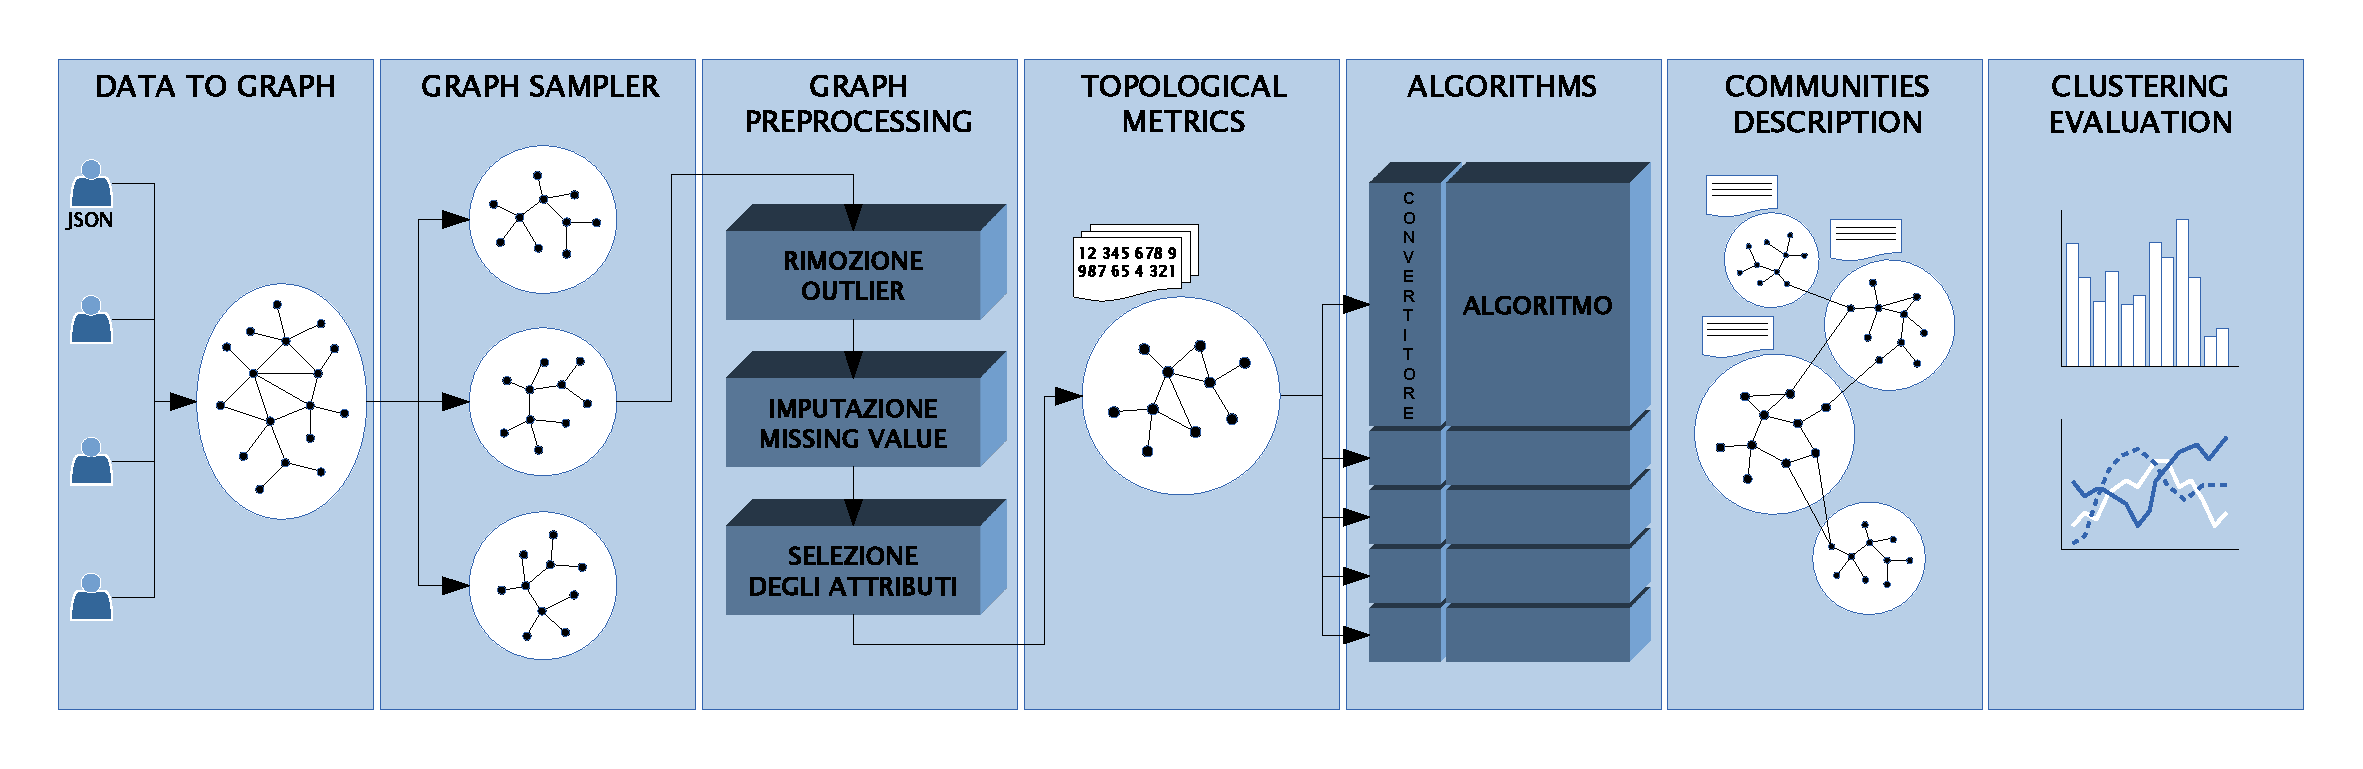
\includegraphics[width=1\textheight]{pictures/workflow.pdf}
    \caption{Workflow modulare dell'architettura}
    \label{fig:framework_flow}
\end{sidewaysfigure}